%! TEX root = main.tex

In conventional numerical methods, the degrees of freedom (i.e., the numbers of model parameters) reflect the model complexity.
And given a numerical method and a model complexity, the workload, time cost, and accuracy are theoretically predictable.
In PINNs, the number of model parameters also determines the model complexity.
However, even with a specific PINN implementation, model complexity may not be the only factor determining the time cost and the accuracy.
The number of training points per batch ($N_{bs}$) apparently also influences the time cost.
One interesting question is whether $N_{bs}$ affects the prediction accuracy or errors.
If yes, then how to choose a proper $N_{bs}$ is a follow-up question. 
If no, it means the time cost does not reflect the PINN methods' performance.
In this section, we would like to examine the relationship between model complexity, batch sizes, error levels, and the time costs.

We first visualize the $L_{2,sp-t}$ errors of $u$ for all cases in figure \ref{fig:tgv2d-re100-err-vs-arch}.
\begin{figure}[hbt!]
    \centering%
    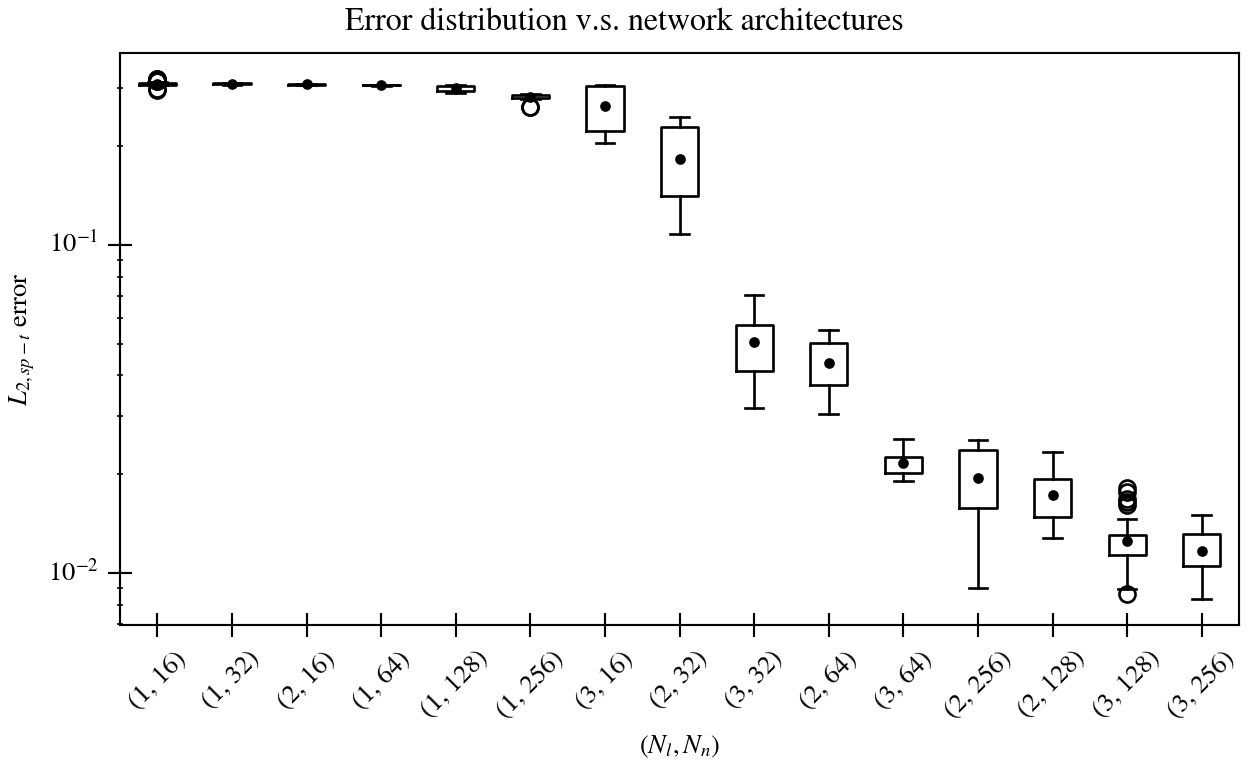
\includegraphics[width=0.95\linewidth]{tgv-2d-re100/err-vs-model-complexity/err-arch-boxplot}
    \caption[%
        PINNs, 2D TGV, $Re=100$: $L_{2,sp-t}$ error v.s. network architecture%
    ]{%
        PINNs, 2D TGV, $Re=100$: $L_{2,sp-t}$ error v.s. network architecture%
    }
    \label{fig:tgv2d-re100-err-vs-arch}
\end{figure}
The $y$-axis is $L_{2,sp-t}$, and $x$-axis denotes the network architectures $(N_l, N_n)$.
The architectures are sorted by their error magnitudes from left to right.
The box plot of each architecture represents the error distributions of different $N_{bs}$ with the same architecture.
We hope this figure can shed some light on how $N_l$, $N_n$, and $N_{bs}$ influence the error levels.
The figure shows that, when $N_l < 2$ or $N_n < 32$, the errors remain at the same level, and $N_{bs}$ does not have any influence.
This may indicate these models are too simple and always underfit the PDEs.
Once the model complexity reaches a certain level, increasing both $N_n$ and $N_l$ helps lower the error levels.
Also, $N_{bs}$ starts to have an effect in these cases.
Nevertheless, if we consider the orders of magnitudes, quantitatively speaking, we don't consider that $N_{bs}$ has a strong impact on the accuracy.
As seen from the figure, model complexity still dominates the error levels. 

It is unclear from figure \ref{fig:tgv2d-re100-err-vs-arch} whether increasing $N_l$ or $N_n$ has a stronger impact on the error levels.
For example, if we are to improve the error level of $(2, 32)$, both $(2, 64)$ and $(3, 32)$ give us similar improvement.
Or, if we are to improve the error of $(2, 64)$, both $(2, 128)$ and $(3, 64)$ give a similar level of errors.
Though increasing $N_l$ or doubling $N_n$ have the same effect in terms of the error levels, their effects in the total number of model parameters are different. 
As seen from equation \eqref{eq:dof-calculator}, the degrees of freedom increase about linearly with $N_l$ but increase proportionally to the square of $N_n$.
In other words, doubling $N_n$ roughly quadruples the number of free parameters, while increasing $N_l$ by one just adds around $N_n^2$ parameters.
Hence, form the viewpoint of computational cost, increasing $N_l$ may be a better choice.

Figure \ref{fig:tgv2d-re100-err-vs-dof} shows a similar box plots but with the $x$-axis being the degrees of freedom.
\begin{figure}[hbt!]
    \centering%
    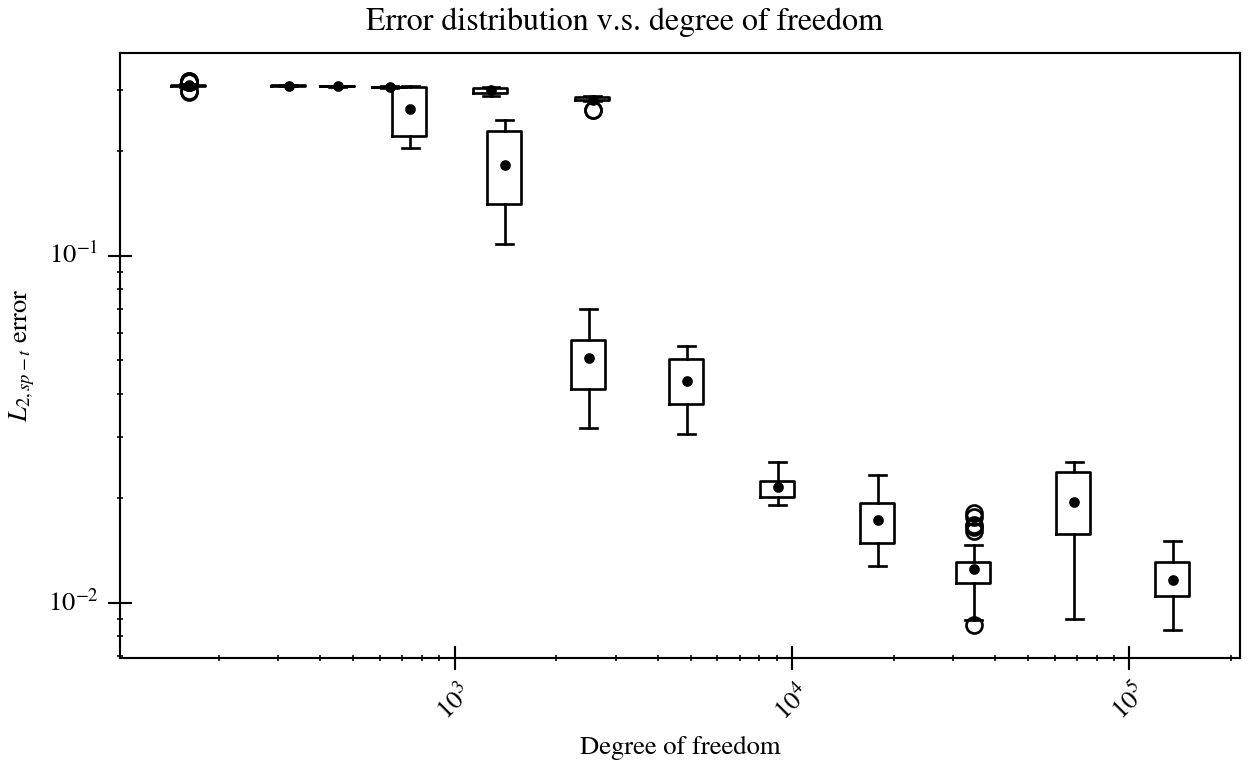
\includegraphics[width=0.95\linewidth]{tgv-2d-re100/err-vs-model-complexity/err-dof-boxplot}
    \caption[%
        PINNs, 2D TGV, $Re=100$: $L_{2,sp-t}$ error v.s. degree of freedom%
    ]{%
        PINNs, 2D TGV, $Re=100$: $L_{2,sp-t}$ error v.s. degree of freedom%
    }
    \label{fig:tgv2d-re100-err-vs-dof}
\end{figure}
From the left portion of the figure, it is obvious that the same number of degrees of freedom does not necessarily give the same accuracy, meaning the model complexity in PINNs can not simply be determined by the number of free parameters in a model.
Also, from the right part of the figure, though increasing the degrees of freedom generally improves the errors, the relationship does not seem to follow a simple monotonically decreasing relationship.
Again, this means the model complexity in PINNs and hence the capability to approximate a complicated flow solution can not be simply determined by the number of free parameters.
This observation also supports the finding that increasing $N_l$ and doubling $N_n$ may have the same effect on the error levels, as the two strategies result in very different numbers of free parameters.

Due to the nonlinearity of PINNs, it is reasonable that the number of free parameters can not be used as a single indicator for how complex an MLP model is.
And to our best knowledge, we have not seen approaches to quantitatively estimate the model complexity.
However, lacking a rigorous understanding of how to evaluate the model complexity in PINNs means, when using PINNs for CFD applications, engineers may not be able to estimate how complicated their PINN models should be to achieve a desired performance.
It further makes it difficult for engineers to evaluate workload, required resources, and costs for engineering projects.

Lastly, figure \ref{fig:tgv2d-re100-err-vs-time} shows the $L_{2,sp-t}$ errors with respect to run times of all cases.
\begin{figure}[hbt!]
    \centering%
    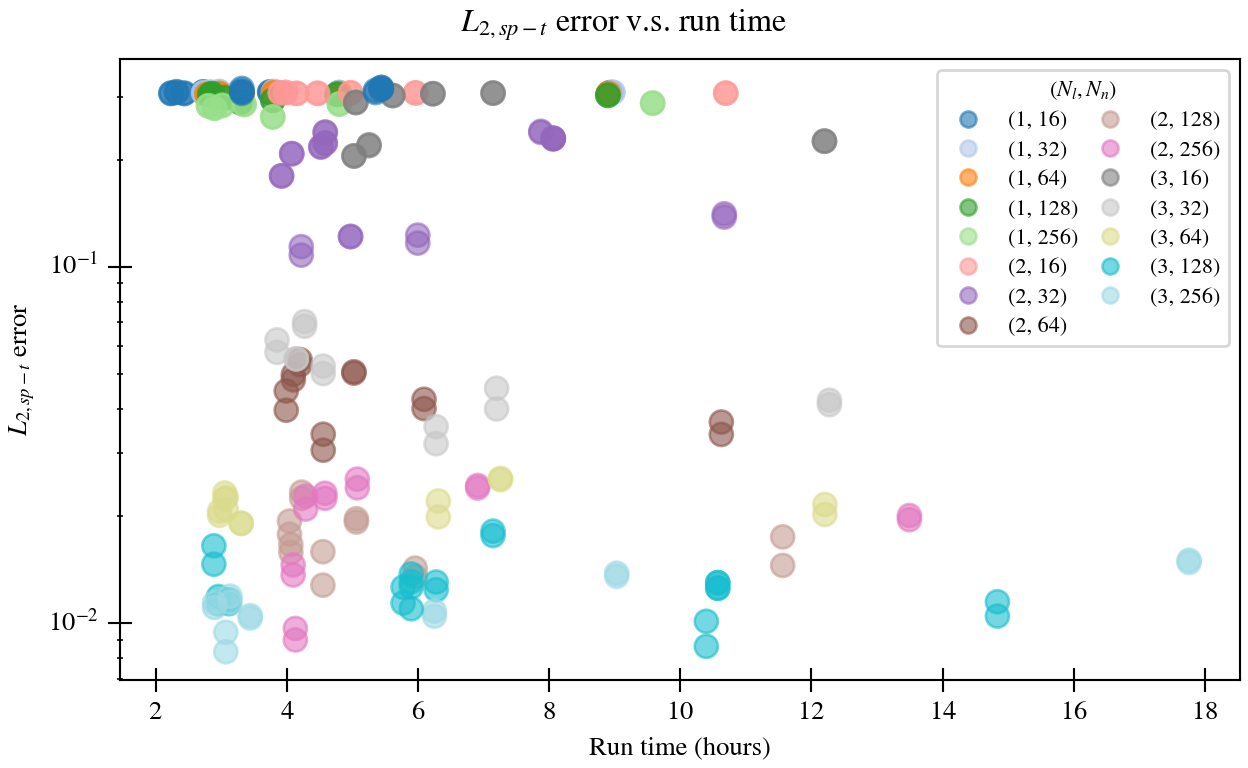
\includegraphics[width=0.95\linewidth]{tgv-2d-re100/err-vs-time/err-time}
    \caption[%
        PINNs, 2D TGV, $Re=100$: $L_{2,sp-t}$ error v.s. run time%
    ]{%
        PINNs, 2D TGV, $Re=100$: $L_{2,sp-t}$ error v.s. run time%
    }
    \label{fig:tgv2d-re100-err-vs-time}
\end{figure}
The colors of dots represent different architectures.
We observed that dots with the same colors are roughly at the same level of errors but are distributed across a wide range of $x$-axis.
It indicates that while $N_{bs}$ has a strong impact on the time costs, it does not have an evident effect on the accuracy.
We did not expect this result because, traditionally in deep learning, using more training data per batch gives a faster convergence and prediction accuracy.
More data per batch means the statistical properties are similar across different batches, and thus the hypersurface does not change significantly from iteration to iteration.
One explanation to the figure \ref{fig:tgv2d-re100-err-vs-time} is that our test cases used too many training points.
The smallest case, $N_{bs}=1024$, might still be big enough for this TGV problem and hence we were not able to see the effect of $N_{bs}$ in the accuracy and convergence rates.
Another explanation is that PINNs are generally insensitive to $N_{bs}$. 
Unfortunately, our test cases are not able to confirm either claim at this point.
If we strictly follow our benchmark results, increasing $N_{bs}$ simply increases the time costs without providing any benefit.
% vim:ft=tex
